\documentclass[a4paper,12pt]{report}
\usepackage{geometry} % Для последующего задания полей
\geometry{a4paper,top=15mm,bottom=20mm,left=10mm,right=10mm}
\usepackage[T2A]{fontenc}	     % Поддержка русских букв
\usepackage[utf8]{inputenc}	     % Кодировка utf8
\usepackage[english, russian]{babel} % Языки: русский, английский
\usepackage{graphicx}                % Подключаем пакет работы с графикой

\renewcommand{\arraystretch}{1.3}

\begin{document}


\section*{Исходные данные}

\begin{table}[h!]
  \renewcommand{\tabcolsep}{0.9em}
  \centering
  \begin{tabular}{cccccccccc}
    (-0.68; -0.26)	& (-4.03; -2.32)	& (-0.72; 0.47)	& (1.25; 0.82)	& (1.27; -0.81)	\\ 
(-3.57; 0.46)	& (3.00; -2.85)	& (-2.19; 2.71)	& (-4.72; 0.48)	& (4.38; 2.77)	\\ 
(1.16; 2.37)	& (-1.04; 2.03)	& (-0.63; 1.74)	& (-0.07; -0.30)	& (-1.55; 1.85)	\\ 
(1.57; -0.10)	& (-0.27; -0.84)	& (-1.92; -0.17)	& (-0.80; -0.27)	& (-0.30; 3.87)	\\ 
(-2.51; -1.20)	& (0.21; 0.36)	& (2.99; 2.78)	& (2.26; 2.43)	& (1.95; 0.79)	\\ 
(3.27; 0.62)	& (-0.40; 2.71)	& (-0.53; 1.01)	& (0.16; 2.11)	& (3.07; 0.47)	\\ 
(-0.87; -2.17)	& (2.41; -0.85)	& (-0.52; -1.54)	& (0.99; -0.26)	& (0.57; 1.41)	\\ 
(1.47; -0.41)	& (5.76; -1.11)	& (-1.16; 0.95)	& (-1.22; -3.60)	& (3.13; 2.46)	\\ 
(0.90; 0.79)	& (0.77; -3.32)	& (-0.80; -1.46)	& (1.48; -0.69)	& (0.18; 0.25)	\\ 
(2.08; 2.50)	& (-0.99; -2.73)	& (-1.33; 1.70)	& (-2.36; -2.75)	& (-1.82; -2.29)	\\ 
	\\ 

  \end{tabular}
  \caption{Исходная выборка}
\end{table}

\begin{figure}[h!] 
  \centering
  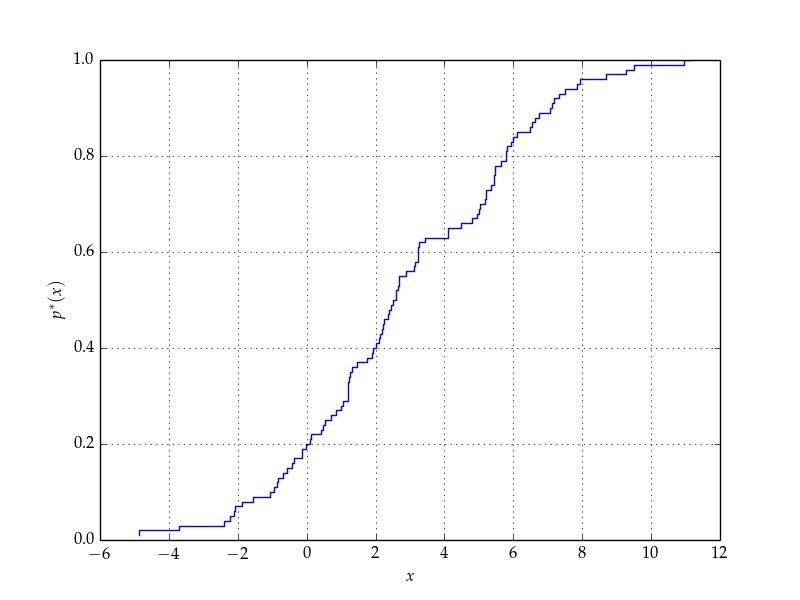
\includegraphics[width=0.8\linewidth]{../pic/sample.png}
  \caption{График гипотетической функции распределения вероятностей}
\end{figure}

\newpage

\section*{Равноинтервальная гистограмма}

\begin{figure}[h!] 
  \centering
  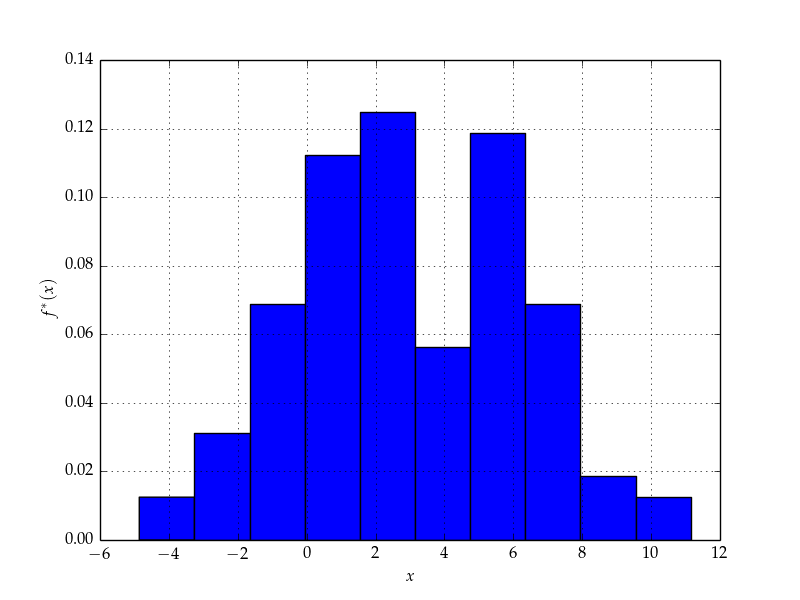
\includegraphics[width=0.8\linewidth]{../pic/stat_series_eq_size.png}
  \caption{Равноинтервальная гистограмма распределения случайной величины}
\end{figure}

\begin{table}[h!]
  \renewcommand{\tabcolsep}{1.6em}
  \centering
  \begin{tabular}{|c|c|c|c|c|c|c|}
    \hline %%% strange bug...
    $ j $	& $ A_j $	& $ B_j $	& $ h_j $	& $ v_j $	& $ p^{*}_j $	& $ f^{*}_j $ \\ \hline
1	& -4.860	& -3.259	& 1.601	& 2	& 0.0200	& 0.0125 \\ \hline
2	& -3.259	& -1.658	& 1.601	& 5	& 0.0500	& 0.0312 \\ \hline
3	& -1.658	& -0.057	& 1.601	& 11	& 0.1100	& 0.0687 \\ \hline
4	& -0.057	& 1.544	& 1.601	& 18	& 0.1800	& 0.1124 \\ \hline
5	& 1.544	& 3.145	& 1.601	& 20	& 0.2000	& 0.1249 \\ \hline
6	& 3.145	& 4.746	& 1.601	& 9	& 0.0900	& 0.0562 \\ \hline
7	& 4.746	& 6.347	& 1.601	& 19	& 0.1900	& 0.1187 \\ \hline
8	& 6.347	& 7.948	& 1.601	& 11	& 0.1100	& 0.0687 \\ \hline
9	& 7.948	& 9.549	& 1.601	& 3	& 0.0300	& 0.0187 \\ \hline
10	& 9.549	& 11.150	& 1.601	& 2	& 0.0200	& 0.0125 \\ \hline
Всего:	&	&	&16.010	&100	&1.0000	& \\ \hline

  \end{tabular}
  \caption{Данные для построения равноинтервальной гистограммы}
\end{table}

\newpage

\section*{Равновероятностная гистограмма}

\begin{figure}[h!] 
  \centering
  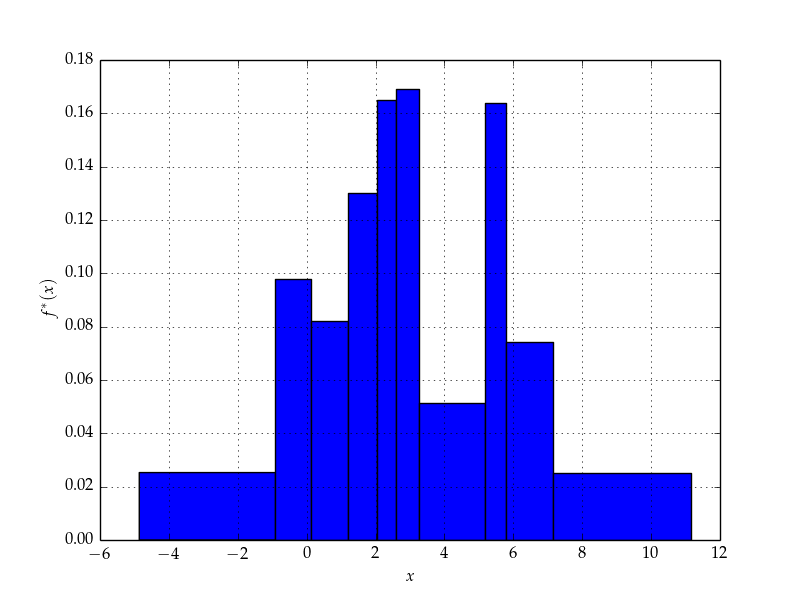
\includegraphics[width=0.8\linewidth]{../pic/stat_series_eq_probability.png}
  \caption{Равновероятностая гистограмма распределения случайной величины}
\end{figure}

\begin{table}[h!]
  \renewcommand{\tabcolsep}{1.6em}
  \centering
  \begin{tabular}{|c|c|c|c|c|c|c|}
    \hline %%% strange bug...
    $ j $	& $ A_j $	& $ B_j $	& $ h_j $	& $ v_j $	& $ p^{*}_j $	& $ f^{*}_j $ \\ \hline
1	& -4.860	& -0.905	& 3.955	& 10	& 0.1000	& 0.0253 \\ \hline
2	& -0.905	& 0.115	& 1.020	& 10	& 0.1000	& 0.0980 \\ \hline
3	& 0.115	& 1.210	& 1.095	& 10	& 0.1000	& 0.0913 \\ \hline
4	& 1.210	& 2.055	& 0.845	& 10	& 0.1000	& 0.1183 \\ \hline
5	& 2.055	& 2.600	& 0.545	& 10	& 0.1000	& 0.1835 \\ \hline
6	& 2.600	& 3.250	& 0.650	& 10	& 0.1000	& 0.1538 \\ \hline
7	& 3.250	& 5.190	& 1.940	& 10	& 0.1000	& 0.0515 \\ \hline
8	& 5.190	& 5.800	& 0.610	& 10	& 0.1000	& 0.1639 \\ \hline
9	& 5.800	& 7.150	& 1.350	& 10	& 0.1000	& 0.0741 \\ \hline
10	& 7.150	& 11.150	& 4.000	& 10	& 0.1000	& 0.0250 \\ \hline
Всего:	&	&	&16.010	&100	&1.0000	& \\ \hline

  \end{tabular}
  \caption{Данные для построения равновероятностной гистограммы}
\end{table}

\newpage

\section*{Гипотеза о равномерном законе \\
  распределения случайной величины}

\begin{figure}[h!] 
  \centering
  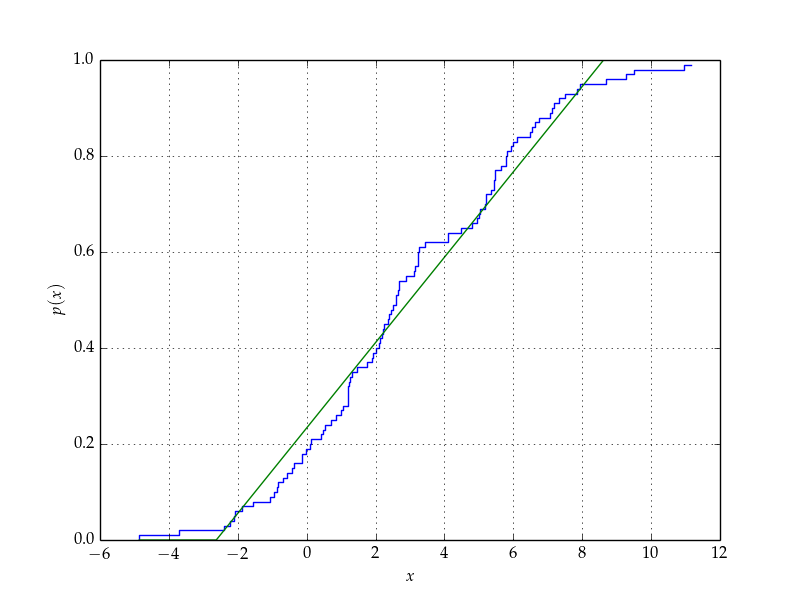
\includegraphics[width=0.8\linewidth]{../pic/sample_uniform.png}
  \caption{Иллюстрация гипотезы о равномерном законе распределения случайной величины}
\end{figure}

\begin{table}[h!]
  \renewcommand{\tabcolsep}{1em}
  \centering
  \begin{tabular}{|c|c|c|c|c|c|c|c|}
    \hline %%% strange bug...
    $ j $	& $ A_j $	& $ B_j $	& $ F_0(A_j) $	& $ F_0(B_j) $	& $ p_j $	& $ p_j^{*} $	& $ \frac{(p^{*}_j - p_j)^2}{p_j} $ \\ \hline
1	& $ -\infty $	& -3.259	& 0.0000	& 0.0000	& 0.0000	& 0.0200	& $ +\infty $ \\ \hline
	&	&	&	&Всего:	&0.0200	&0.0000	&$ +\infty $ \\ \hline

  \end{tabular}
  \caption{Промежуточные вычисления критерия согласия Пирсона}
\end{table}

\newpage

\section*{Гипотеза об экспоненциальном законе \\
  распределения случайной величины}

\begin{figure}[h!] 
  \centering
  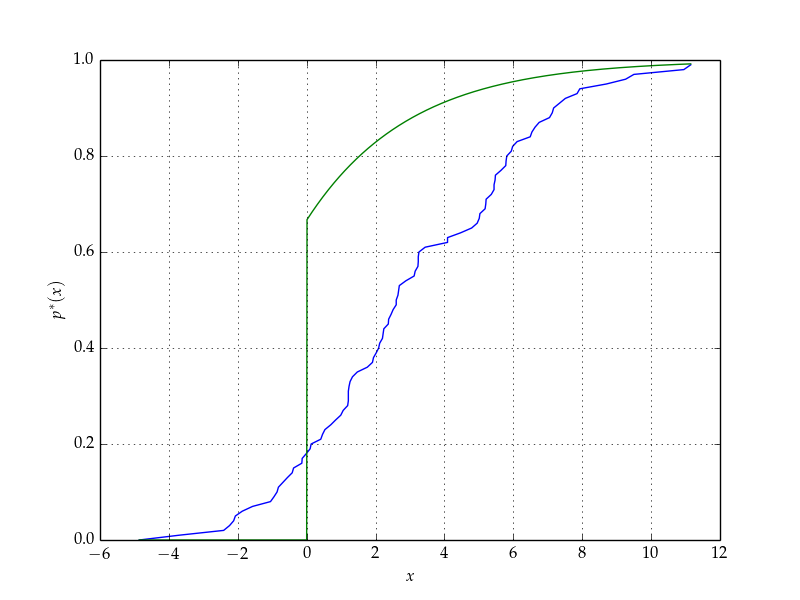
\includegraphics[width=0.8\linewidth]{../pic/sample_exponential.png}
  \caption{Иллюстрация гипотезы об экспоненциальном законе распределения случайной величины}
\end{figure}

\begin{table}[h!]
  \renewcommand{\tabcolsep}{1em}
  \centering
  \begin{tabular}{|c|c|c|c|c|c|c|c|}
    \hline %%% strange bug...
    $ j $	& $ A_j $	& $ B_j $	& $ F_0(A_j) $	& $ F_0(B_j) $	& $ p_j $	& $ p_j^{*} $	& $ \frac{(p^{*}_j - p_j)^2}{p_j} $ \\ \hline
1	& $ -\infty $	& -3.259	& 0.0000	& 0.0000	& 0.0000	& 0.0200	& $ +\infty $ \\ \hline
	&	&	&	&Всего:	&0.0200	&0.0000	&$ +\infty $ \\ \hline

  \end{tabular}
  \caption{Промежуточные вычисления критерия согласия Пирсона для экспоненциального распределения}
\end{table}

\newpage


\section*{Гипотеза о нормальном законе \\
  распределения случайной величины}

\begin{figure}[h!] 
  \centering
  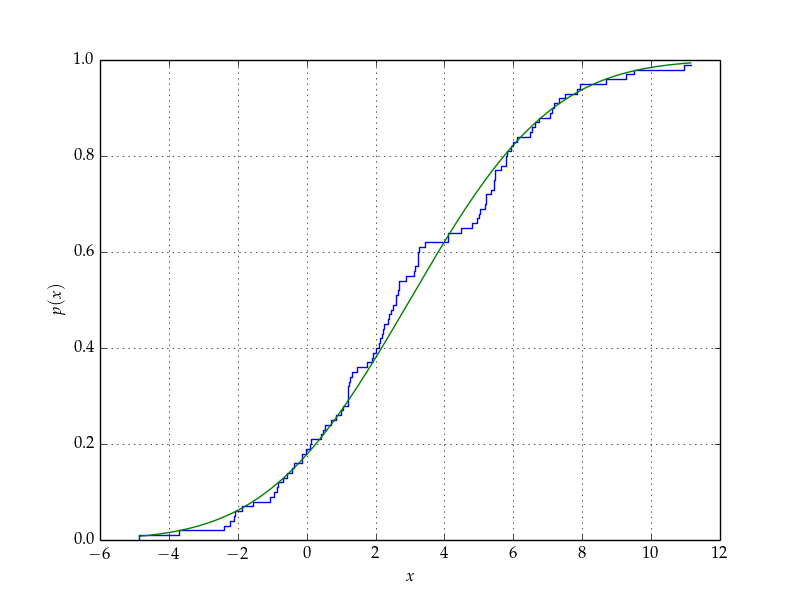
\includegraphics[width=0.8\linewidth]{../pic/sample_normal.png}
  \caption{Иллюстрация гипотезы о нормальном законе распределения случайной величины}
\end{figure}

\begin{table}[h!]
  \renewcommand{\tabcolsep}{1em}
  \centering
  \begin{tabular}{|c|c|c|c|c|c|c|c|}
    \hline %%% strange bug...
    $ j $	& $ A_j $	& $ B_j $	& $ F_0(A_j) $	& $ F_0(B_j) $	& $ p_j $	& $ p_j^{*} $	& $ \frac{(p^{*}_j - p_j)^2}{p_j} $ \\ \hline
1	& $ -\infty $	& -3.259	& 0.0000	& 0.0269	& 0.0269	& 0.0200	& 0.0018 \\ \hline
2	& -3.259	& -1.658	& 0.0269	& 0.0757	& 0.0487	& 0.0500	& 0.0000 \\ \hline
3	& -1.658	& -0.057	& 0.0757	& 0.1732	& 0.0975	& 0.1100	& 0.0016 \\ \hline
4	& -0.057	& 1.544	& 0.1732	& 0.3268	& 0.1536	& 0.1800	& 0.0045 \\ \hline
5	& 1.544	& 3.145	& 0.3268	& 0.5188	& 0.1921	& 0.2000	& 0.0003 \\ \hline
6	& 3.145	& 4.746	& 0.5188	& 0.7055	& 0.1866	& 0.0900	& 0.0500 \\ \hline
7	& 4.746	& 6.347	& 0.7055	& 0.8492	& 0.1438	& 0.1900	& 0.0149 \\ \hline
8	& 6.347	& 7.948	& 0.8492	& 0.9365	& 0.0873	& 0.1100	& 0.0059 \\ \hline
9	& 7.948	& 9.549	& 0.9365	& 0.9783	& 0.0418	& 0.0300	& 0.0033 \\ \hline
10	& 9.549	& $ +\infty $	& 0.9783	& 1.0000	& 0.0217	& 0.0200	& 0.0001 \\ \hline
	&	&	&	&Всего:	&1.0000	&1.0000	&0.0826 \\ \hline

  \end{tabular}
  \caption{Промежуточные вычисления критерия согласия Пирсона}
\end{table}

\newpage


\end{document}